 \documentclass[11pt]{article}  

%%%%%%%% PREÁMBULO %%%%%%%%%%%%
\title{CG}

\usepackage{tikz}
\usepackage[spanish]{babel} %Indica que escribiremos en español
\usepackage[utf8]{inputenc} %Indica qué codificación se está usando ISO-8859-1(latin1)  o utf8 
\usepackage{amsmath}
\usepackage{amssymb} % Símbolos matematicos (por lo tanto)
\usepackage{graphicx} % Incluir imágenes en LaTeX
\usepackage{color} % Para colorear texto
\usepackage{array}
\usepackage{multirow}
\usepackage{enumitem}
\usepackage{subcaption}
\usepackage{graphicx}
\usepackage{tabu}
\usepackage{listings} % Para usar código fuente
\usepackage{xcolor}

\definecolor{codegreen}{rgb}{0,0.6,0}
\definecolor{codegray}{rgb}{0.5,0.5,0.5}
\definecolor{codepurple}{rgb}{0.58,0,0.82}
\definecolor{backcolour}{rgb}{0.95,0.95,0.92}
\definecolor{lightgray}{rgb}{0.95, 0.95, 0.95}
\definecolor{darkgray}{rgb}{0.4, 0.4, 0.4}
%\definecolor{purple}{rgb}{0.65, 0.12, 0.82}
\definecolor{editorGray}{rgb}{0.95, 0.95, 0.95}
\definecolor{editorOcher}{rgb}{1, 0.5, 0} % #FF7F00 -> rgb(239, 169, 0)
\definecolor{editorGreen}{rgb}{0, 0.5, 0} % #007C00 -> rgb(0, 124, 0)
\definecolor{orange}{rgb}{1,0.45,0.13}		
\definecolor{olive}{rgb}{0.17,0.59,0.20}
\definecolor{brown}{rgb}{0.69,0.31,0.31}
\definecolor{purple}{rgb}{0.38,0.18,0.81}
\definecolor{lightblue}{rgb}{0.1,0.57,0.7}
\definecolor{lightred}{rgb}{1,0.4,0.5}

\lstdefinestyle{mystyle}{
    backgroundcolor=\color{backcolour},   
    commentstyle=\color{codegreen},
    keywordstyle=\color{magenta},
    numberstyle=\tiny\color{codegray},
    stringstyle=\color{codepurple},
    basicstyle=\ttfamily\footnotesize,
    breakatwhitespace=false,         
    breaklines=true,                 
    captionpos=b,                    
    keepspaces=true,                 
    numbers=left,                    
    numbersep=5pt,                  
    showspaces=false,                
    showstringspaces=false,
    showtabs=false,                  
    tabsize=2
}
% JavaScript
\lstdefinelanguage{JavaScript}{
  morekeywords={this, typeof, new, true, false, catch, function, return, null, catch, switch, var, if, in, while, do, else, case, break, let, const, :},
  morecomment=[s]{/*}{*/},
  morecomment=[l]//,
  morestring=[b]",
  morestring=[b]'
}

\lstdefinelanguage{HTML5}{
  language=html,
  sensitive=true,	
  alsoletter={<>=-},	
  morecomment=[s]{<!-}{-->},
  tag=[s],
  otherkeywords={
  % General
  >,
  % Standard tags
	<!DOCTYPE,
  </html, <html, <head, <title, </title, <style, </style, <link, </head, <meta, />,
	% body
	</body, <body,
	% Divs
	</div, <div, </div>, 
	% Paragraphs
	</p, <p, </p>,
	% scripts
	</script, <script,
  % More tags...
  <canvas, /canvas>, <svg, <rect, <animateTransform, </rect>, </svg>, <video, <source, <iframe, </iframe>, </video>, <image, </image>, <header, </header, <article, </article, <input,<button, </button, <label, </label, <br,/br>
  },
  ndkeywords={
  % General
  =,
  % HTML attributes
  charset=, src=, id=, width=, height=, style=, type=, rel=, href=,
  % SVG attributes
  fill=, attributeName=, begin=, dur=, from=, to=, poster=, controls=, x=, y=, repeatCount=, xlink:href=,
  % properties
  margin:, padding:, background-image:, border:, top:, left:, position:, width:, height:, margin-top:, margin-bottom:, font-size:, line-height:,
	% CSS3 properties
  transform:, -moz-transform:, -webkit-transform:,
  animation:, -webkit-animation:,
  transition:,  transition-duration:, transition-property:, transition-timing-function:,
  }
}
\lstdefinestyle{htmlcssjs} {%
  % General design
%  backgroundcolor=\color{editorGray},
  backgroundcolor=\color{backcolour},   
  basicstyle=\ttfamily\footnotesize,
  basicstyle={\footnotesize\ttfamily},   
  frame=b,
  % line-numbers
  xleftmargin={0.75cm},
  numbers=left,
  stepnumber=1,
  firstnumber=1,
  numberfirstline=true,	
  % Code design
  identifierstyle=\color{black},
  keywordstyle=\color{blue}\bfseries,
  ndkeywordstyle=\color{editorGreen}\bfseries,
  stringstyle=\color{editorOcher}\ttfamily,
  commentstyle=\color{brown}\ttfamily,
  % Code
  language=HTML5,
  alsolanguage=JavaScript,
  alsodigit={.:;},	
  tabsize=2,
  showtabs=false,
  showspaces=false,
  showstringspaces=false,
  extendedchars=true,
  breaklines=true,
  % German umlauts
  literate=%
  {Ö}{{\"O}}1
  {Ä}{{\"A}}1
  {Ü}{{\"U}}1
  {ß}{{\ss}}1
  {ü}{{\"u}}1
  {ä}{{\"a}}1
  {ö}{{\"o}}1
}


\lstset{style=mystyle}

\definecolor{dkgreen}{rgb}{0,0.6,0} % Definimos colores para usar en el código
\definecolor{gray}{rgb}{0.5,0.5,0.5} 
% configuración para el lenguaje que queramos utilizar
\lstset{language=Matlab,
   keywords={break,case,catch,continue,else,elseif,end,for,function,
      global,if,otherwise,persistent,return,switch,try,while},
   basicstyle=\ttfamily,
   keywordstyle=\color{blue},
   commentstyle=\color{red},
   stringstyle=\color{dkgreen},
   %numbers=left,
   %numberstyle=\tiny\color{gray},
   %stepnumber=1,
   numbersep=10pt,
   backgroundcolor=\color{white},
   tabsize=4,
   showspaces=false,
   showstringspaces=false}



\newcommand{\sen}{\operatorname{\sen}}	% Definimos el comando \sen para el seno
%en español

\usepackage{float} %Podemos usar el especificador [H] en las figuras para que se
% queden donde queramos
\usepackage{capt-of} % Permite usar etiquetas fuera de elementos flotantes
% (etiquetas de figuras)
\usepackage{sidecap} % Para poner el texto de las imágenes al lado
	\sidecaptionvpos{figure}{c} % Para que el texto se alinie al centro vertical
\usepackage{caption} % Para poder quitar numeracion de figuras
\usepackage{sidecap} % Para poner el texto de las imágenes al lado
	\sidecaptionvpos{figure}{c} % Para que el texto se alinie al centro vertical
\usepackage{caption} % Para poder quitar numeracion de figuras
\usepackage{commath} % funcionalidades extras para diferenciales,
\usepackage{commath} % funcionalidades extras para diferenciales, integrales,
% etc (\od, \dif, etc)
\usepackage{cancel} % para cancelar expresiones (\cancelto{0}{x})
\usepackage{subcaption}
 
\usepackage{anysize} 					% Para personalizar el anchhttps://www.overleaf.com/project/5c0fb40aa77c632fc1f86e58o de  los márgenes
\marginsize{2cm}{2cm}{2cm}{2cm} % Izquierda, derecha, arriba, abajo

\usepackage{appendix}
\renewcommand{\appendixname}{Apéndices}
\renewcommand{\appendixtocname}{Apéndices}
\renewcommand{\appendixpagename}{Apéndices} 

% Para que las referencias sean hipervínculos a las figuras o ecuaciones y
% aparezcan en color
\usepackage[colorlinks=true,plainpages=true,citecolor=blue,linkcolor=blue]{hyperref}
%\usepackage{hyperref} 
% Para agregar encabezado y pie de página
\usepackage{fancyhdr} 
\pagestyle{fancy}
\fancyhf{}
\fancyhead[L]{\footnotesize UNSA} %encabezado izquierda
\fancyhead[R]{\footnotesize EPCC}   % dereecha
\fancyfoot[R]{\footnotesize CG}  % Pie derecha
\fancyfoot[C]{\thepage}  % centro
\fancyfoot[L]{\footnotesize Ciencia de la Computación}  %izquierda


\title{Trabajo}

%%%%%%%% TERMINA PREÁMBULO %%%%%%%%%%%%

\begin{document}

%%%%%%%%%%%%%%%%%%%%%%%%%%%%%%%%%% PORTADA %%%%%%%%%%%%%%%%%%%%%%%%%%%%%%%%%%%%%%%%%%%%
																					%%%
\begin{center}																		%%%
\newcommand{\HRule}{\rule{\linewidth}{0.5mm}}									%%%\left
 																					%%%
\begin{minipage}{0.5\textwidth} \begin{flushleft}

\includegraphics[scale = 0.4]{img/cslogo.png}
\end{flushleft}\end{minipage}
\begin{minipage}{0.48\textwidth} \begin{flushright}

\includegraphics[scale = 0.3]{img/logounsa.png}
\end{flushright}\end{minipage}

													 								%%%
\vspace*{-1.5cm}								%%%
																					%%%	
\textsc{\huge UNIVERSIDAD NACIONAL DE\\ SAN AGUSTÍN \vspace{5px}}\\[1.5cm]	

\textsc{\LARGE Facultad de Ingeniería de Producción y Servicios}\\[1.5cm]													%%%

\begin{minipage}{0.9\textwidth} 
\begin{center}																					%%%
\textsc{\LARGE Ciencia de la Computación}
\end{center}
\end{minipage}\\[0.5cm]
%%%
    																				%%%
 			\vspace*{1cm}																		%%%
																					%%%
\HRule \\[0.4cm]																	%%%
{ \huge \bfseries Laboratorio 3
}\\[0.4cm]	%%%
 																					%%%
\HRule \\[1.5cm]																	%%%
 																				%%%
																					%%%
\begin{minipage}{0.46\textwidth}													%%%
\begin{flushleft} \large															%%%
\centering

\textbf{ALUMNOS:}\\
Pfuturi Huisa, Oscar David\\
Quispe Menor, Hermogenes\\
Quiñonez Lopez, Efrain German\\
Fernandez Mamani, Brayan Gino\\
Santos Apaza, Yordy Williams

\	\vfill

\textbf{DOCENTE:} \\
MSc. Vicente Machaca Arceda

\	\vfill

\textbf{CURSO:}\\
Computación Gráfica

%\vspace*{2cm}	
            													%%%
										 						%%%
\end{flushleft}																		%%%
\end{minipage}		
																%%%
\begin{minipage}{0.70\textwidth}		
\vspace{-0.6cm}											%%%
																	%%%
\end{minipage}	
\vspace*{1cm}
%\begin{flushleft}
 	
%\end{flushleft}
%%%																		%%%
\vspace{3cm} 																				
\begin{center}																					
{\large \today}																	%%%
 			\end{center}												  						
\end{center}							 								\newpage
\newpage																

\tableofcontents 

\newpage
%%%%%%%%%%%%%%%%%%%%%%%%%%%%%%%%%%%%%%%%%%%%%%%%%%%%%%%%%%%%%%%%
\section{Github}

\begin{itemize}
    \item \url{https://github.com/oscar-pfuturi-h/Comp-Grafica/tree/main/practica_3}
\end{itemize}

\section{Temática}
La temática escogida para este trabajo fue medieval. Dado a la tematica escogida y que se representa por la ficción, los elementos creados son 

\begin{itemize}
    \item Castillo
    \item Torres
    \item Dragones
\end{itemize}

\section{Funciones}

\subsection{Crear Castillo}
Para la creación del castillo, se modulo en varias funciones, tales son:

\

la creación de las torres:

\begin{lstlisting}[language=javascript,frame=single]
function CrearCastillo() {
    var paredMaterial = new THREE.MeshLambertMaterial({ color: 0xeeeeee });
    var roofMaterial = new THREE.MeshLambertMaterial({ color: 0xd50000 });

    function crearTorre(alturaT, alturaR, radio) {
        var torre = new THREE.Mesh(new THREE.CylinderGeometry(radio, radio, alturaT, 30), paredMaterial);
        torre.castShadow = true;
        torre.position.y = 5;

        var roof = new THREE.Mesh(new THREE.CylinderGeometry(0, radio, alturaR, 30), roofMaterial);
        roof.castShadow = true;
        roof.position.y = alturaT - (alturaT / 2 - alturaR / 2);
        torre.add(roof);

        return torre;
\end{lstlisting}

La creación de las paredes:

\begin{lstlisting}[language=javascript,frame=single]
function crearpared(paredWidth) {
    var paredHeight = 38;
    var paredDepth = 10;
    var paredGeometry = new THREE.CubeGeometry(paredWidth, paredHeight, paredDepth);
    var pared = new THREE.Mesh(paredGeometry, paredMaterial);
    pared.castShadow = true;
    pared.position.y = paredHeight / 2;
    var battlementSize = 4;
    var battlementGeometry = new THREE.CubeGeometry(battlementSize, battlementSize, battlementSize);

    for (var x = 13 + -(paredWidth / 2) + battlementSize / 2; x < paredWidth / 2 - 10; x += battlementSize * 2) {
        var battlement = new THREE.Mesh(battlementGeometry, paredMaterial);
        battlement.castShadow = true;
        battlement.position.set(x, paredHeight / 2 + battlementSize / 2, paredDepth / 2 - battlementSize / 2);
        pared.add(battlement);
}
\end{lstlisting}

La creación de la entrada:

\begin{lstlisting}[language=javascript,frame=single]
function crearGate() {
    var gateBuildingWidth = 50;
    var gateBuildingHeight = 50;
    var gateBuildingDepth = 40;

    var gateBuilding = new THREE.Mesh(new THREE.CubeGeometry(gateBuildingWidth, gateBuildingHeight, gateBuildingDepth), paredMaterial);
    gateBuilding.castShadow = true;

    gateBuilding.position.y = gateBuildingHeight / 2;

    var ellipse = new THREE.EllipseCurve(0, 0, 20, 30, 0, Math.PI);
    var ellipsePath = new THREE.Path(ellipse.getPoints(50));

    var gateGeometry = new THREE.ShapeGeometry(ellipsePath.toShapes()[0]);
    var gateMaterial = new THREE.MeshBasicMaterial({ color: 0x4e3100 });

    var outerGate = new THREE.Mesh(gateGeometry, gateMaterial);
    var innerGate = new THREE.Mesh(gateGeometry, gateMaterial);

\end{lstlisting}


\subsection{Funciones auxiliares y básicas para crear dragones y algunos objetos}
Al diseñar varios objetos complejos nos dimos cuenta la gran cantidad de código duplicado que encontramos al crear algún objeto compuesto, por lo cual, al igual que trabajar con VTK, Three js al estar basado en el lenguaje de programación Javascript, nos permite abstraer algunos conceptos para crear funciones que nos ayudaran a crear de forma mas rápida y ordenada nuevos objetos.\\

A continuación están algunas de las funciones que nos ayudaron a crear nuestro trabajo de laboratorio, tenemos funciones que nos transforman valores para manejarlos fácilmente(2 primeras funciones) y luego tenemos las demás funciones que se encargan de crear objetos de three js configurables que de forma fácil, solo pasando parámetros los obtenemos para poder agregarlos a nuestra escena general.\\


\begin{lstlisting}[language=javascript,frame=single]
 const gradosARadianes = deg => (deg * Math.PI) / 180.0;
 function hexToRgb(hex) {...}
 function crear_cubo(x, y, z, color){...}
 function crear_cilindro(x, y, z, r, color) {...}
 function crear_esfera(r, x, y, color, opacity) {...}
 function crear_cono(rtop, rbotton, altura, resolucion, color) {...}
 function crear_cola(scale, color_base, color_alas) {...}
 function crear_cabeza(color_base, color_alas) {...}
\end{lstlisting}
Luego tenemos la función Dragón la que se encarga de usar las funciones ya descritas para crear cada objeto, algo muy útil en Three js que no encontramos de forma fácil en la librería VTK es agregar un objeto X a otro objeto Y, lo cual nos da como resultado que el objeto X posee el desplazamiento respecto a su objeto Padre, en este caso seria Objeto Y, de forma fácil no nos tenemos que preocupar al momento de generar movimiento a cada articulación.
\\


\begin{lstlisting}[language=javascript,frame=single]
 function dragon(color_base, color_alas) {
    let dragon = new THREE.Object3D();
    ...
    //ADD
    dragon.add(body);
    dragon.add(ala1); dragon.add(ala2);
    dragon.add(p1); dragon.add(p2); dragon.add(p3); dragon.add(p4);
    dragon.add(cola);
    dragon.add(cabeza);
    return dragon;
}
\end{lstlisting}
Para crear la casa básica, de igual manera se usa las distintas funciones para armar poco a poco la edificación.
\section{Resultados}
\


\begin{figure}[H]
    \centering    
    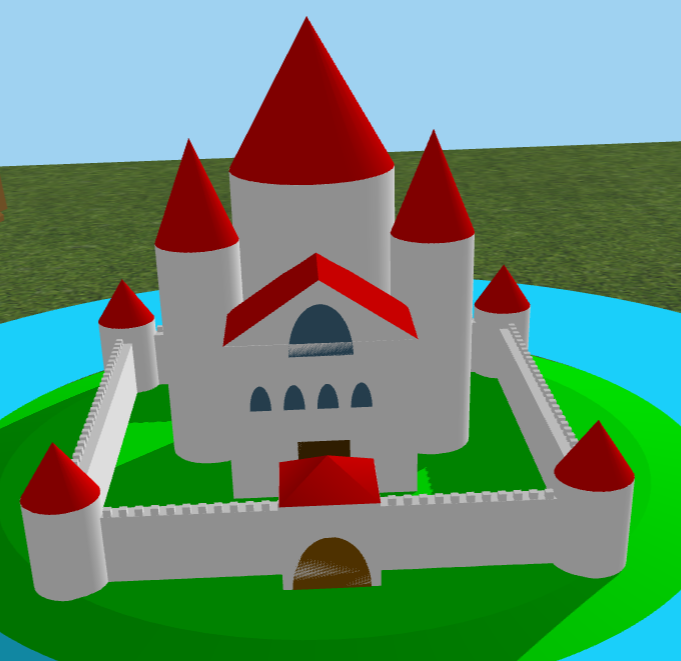
\includegraphics[scale=0.7]{img/castillo.png}
    \caption{Castillo}
\end{figure}

\begin{figure}[H]
    \centering    
    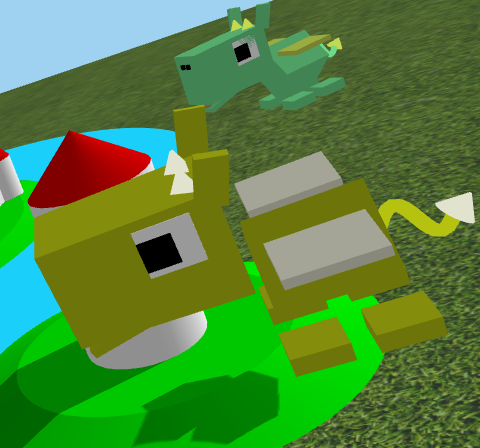
\includegraphics[scale=0.7]{img/dragones.PNG}
    \caption{Dragones}
\end{figure}

\begin{figure}[H]
    \centering    
    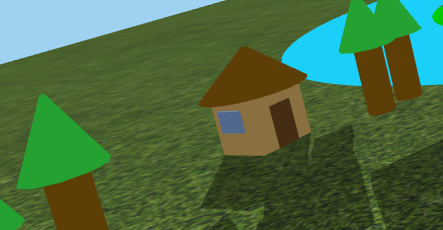
\includegraphics[scale=0.7]{img/casa.PNG}
    \caption{Casa básica}
\end{figure}

\begin{figure}[H]
    \centering    
    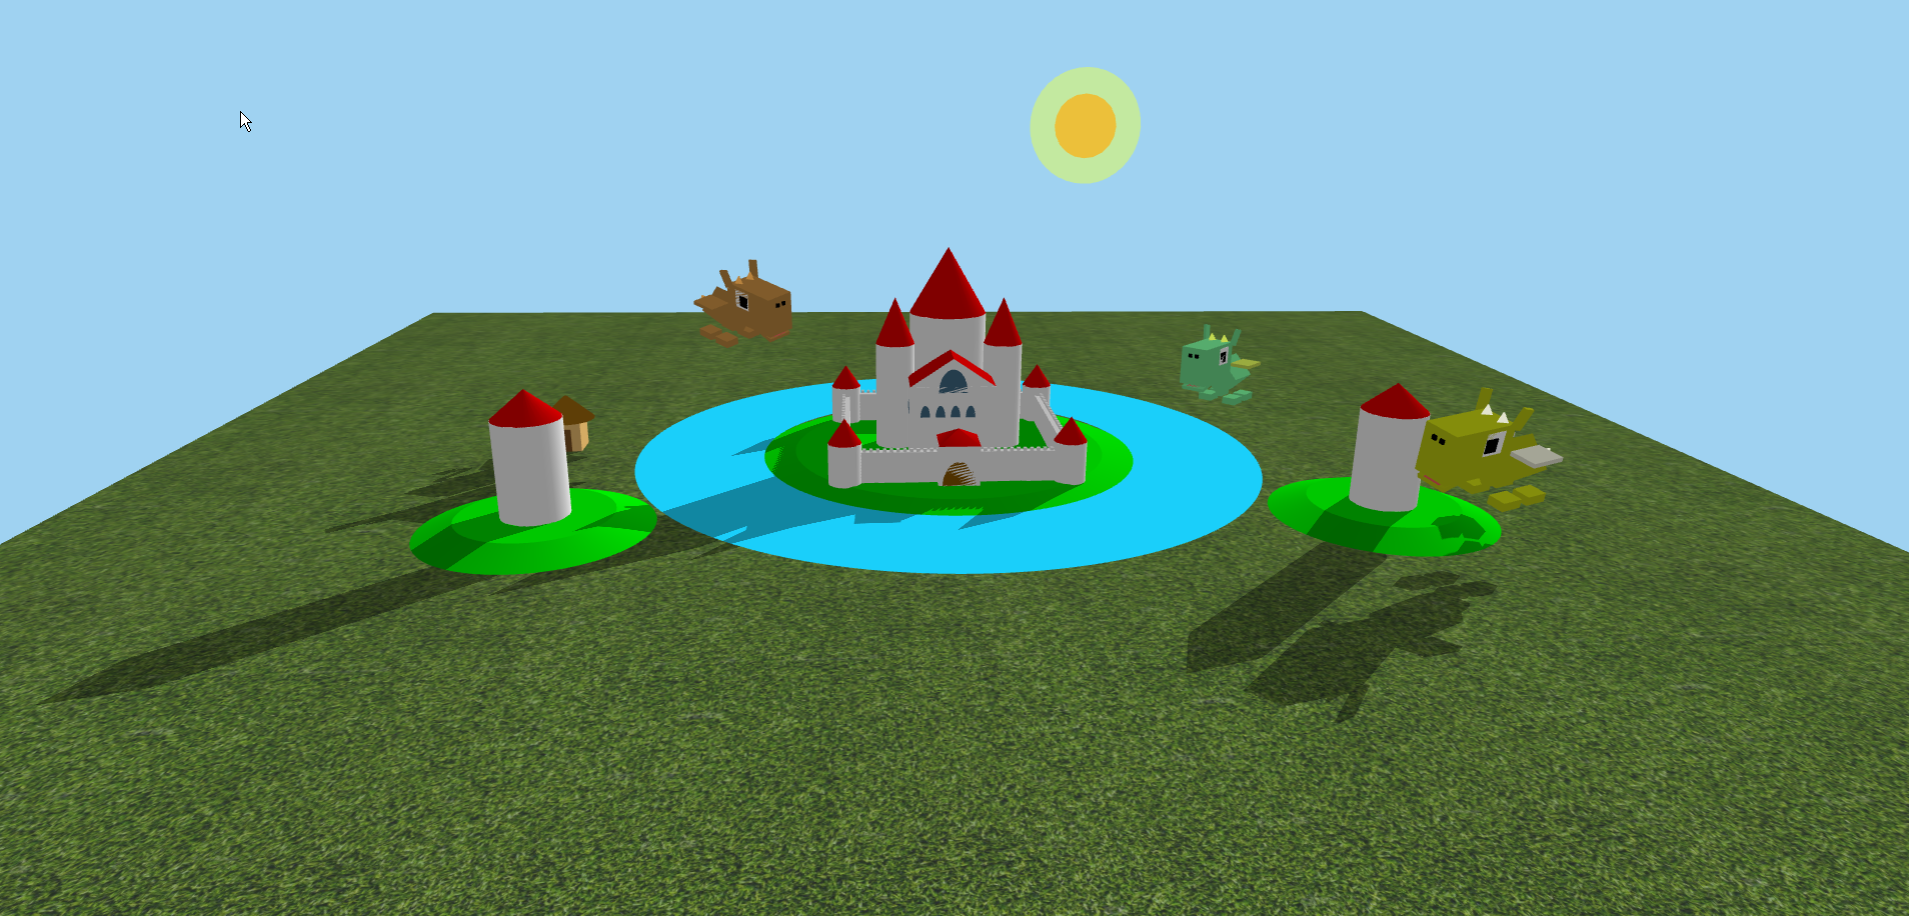
\includegraphics[scale=0.42]{img/full.png}
    \caption{Panorama completo}
\end{figure}

\end{document}